\documentclass[11pt]{article}
\usepackage[margin=1in]{geometry}
\usepackage{amsmath,amssymb,amsthm,booktabs,graphicx,hyperref,xcolor,tikz}
\usetikzlibrary{arrows.meta,positioning}
\usepackage[numbers]{natbib}
\usepackage{caption}
\newtheorem{theorem}{Theorem}
\newcommand{\todo}[1]{\textcolor{red}{[TODO: #1]}}
\newcommand{\E}{\mathcal{E}}
% RULE: every empirical number below is a macro from generated/numbers.tex, or a table or figure in generated/,
% produced from provenance-stamped results/*.json by scripts/make_paper1.py and scripts/plot_*.py.
% Never type a result by hand. Protocol: EVALUATION.md. Pre-registrations: papers/latent-hindsight-planning/*_preregistration.md.
% generated by scripts/make_paper1.py -- DO NOT EDIT
% provenance theory_hindsight: commits ['6e7a3ea'], dirty=False, seeds/runs=3
% provenance realdata_hindsight: commits ['0274fa0', '0603271'], dirty=False, seeds/runs=3
% provenance sealed_v3_hybrid: commits ['41de4eb'], dirty=False, seeds/runs=3
% provenance mujoco_v3_main: commits ['9398e5f', 'e554525'], dirty=False, seeds/runs=3
% provenance mujoco_v3_ksweep: commits ['a406392', 'b7d8f7a'], dirty=False, seeds/runs=3
% provenance mujoco_v3_rho: commits ['e554525'], dirty=False, seeds/runs=3
% provenance mujoco_v3_noise2: commits ['3c40ae8'], dirty=False, seeds/runs=3
% provenance identification_v4: commits ['0ec4d38'], dirty=False, seeds/runs=3
% provenance diag_confound: commits ['eb344b9'], dirty=False, seeds/runs=1
% provenance river: commits ['a36ff57'], dirty=False, seeds/runs=3
% provenance river_v2: commits ['e2950d0'], dirty=False, seeds/runs=3
% provenance throw: commits ['55e206d', '72a91db'], dirty=False, seeds/runs=3
% provenance mujoco_v3_delay: commits ['12fca02', '1db147f', 'c1ae4eb'], dirty=False, seeds/runs=12
% provenance hier_main: commits ['484bf30', '5e36910', '789a0d5'], dirty=False, seeds/runs=3
% provenance latency: commits ['5e36910'], dirty=False, seeds/runs=2
\newcommand{\cfDipPin}{0.000}
\newcommand{\cfDipStd}{-0.286}
\newcommand{\cfRPin}{0.996}
\newcommand{\dlCapture}{66.4\%}
\newcommand{\dlGainTwenty}{36.7\%}
\newcommand{\dlGainZero}{2.3\%}
\newcommand{\dlOracleTwenty}{0.447}
\newcommand{\dlOracleZero}{0.975}
\newcommand{\dlPostTwenty}{0.633}
\newcommand{\dlPostVsSgdTwenty}{0.722}
\newcommand{\dlPostVsSgdZero}{0.991}
\newcommand{\dlPostZero}{0.977}
\newcommand{\dlSgdTwenty}{0.876}
\newcommand{\dlSgdZero}{0.986}
\newcommand{\hiCapture}{90.4\%}
\newcommand{\hiDiffBoth}{+0.31}
\newcommand{\hiDiffFresh}{-0.11}
\newcommand{\hiDiffHiBoth}{+0.39}
\newcommand{\hiDiffHiFresh}{-0.01}
\newcommand{\hiDiffHiNone}{+0.00}
\newcommand{\hiDiffHiWind}{+0.28}
\newcommand{\hiDiffLoBoth}{+0.24}
\newcommand{\hiDiffLoFresh}{-0.20}
\newcommand{\hiDiffLoNone}{+0.00}
\newcommand{\hiDiffLoWind}{+0.15}
\newcommand{\hiDiffNone}{+0.00}
\newcommand{\hiDiffWind}{+0.21}
\newcommand{\hiEpisodes}{150}
\newcommand{\hiFlatBoth}{0.04}
\newcommand{\hiFlatFresh}{0.01}
\newcommand{\hiFlatHindBoth}{0.00}
\newcommand{\hiFlatHindFresh}{0.00}
\newcommand{\hiFlatHindNone}{0.00}
\newcommand{\hiFlatHindWind}{0.00}
\newcommand{\hiFlatNone}{0.41}
\newcommand{\hiFlatWind}{0.09}
\newcommand{\hiFwdBoth}{0.55}
\newcommand{\hiFwdFresh}{0.36}
\newcommand{\hiFwdNone}{1.00}
\newcommand{\hiFwdWind}{0.73}
\newcommand{\hiHindBoth}{0.86}
\newcommand{\hiHindFresh}{0.25}
\newcommand{\hiHindNone}{1.00}
\newcommand{\hiHindWind}{0.94}
\newcommand{\hiOracleBoth}{0.89}
\newcommand{\hiOracleFresh}{0.94}
\newcommand{\hiOracleNone}{1.00}
\newcommand{\hiOracleWind}{0.98}
\newcommand{\hiPfBoth}{0.83}
\newcommand{\hiPfFresh}{0.37}
\newcommand{\hiPfNone}{1.00}
\newcommand{\hiPfWind}{0.95}
\newcommand{\hiResidBoth}{0.77}
\newcommand{\hiResidFresh}{0.39}
\newcommand{\hiResidNone}{1.00}
\newcommand{\hiResidWind}{0.95}
\newcommand{\hiSgdBoth}{0.64}
\newcommand{\hiSgdFresh}{0.37}
\newcommand{\hiSgdNone}{1.00}
\newcommand{\hiSgdWind}{0.84}
\newcommand{\idPredDip}{0.138}
\newcommand{\idPredEnd}{0.888}
\newcommand{\idPredTwenty}{0.773}
\newcommand{\idWindTwenty}{0.837}
\newcommand{\ksGainForty}{34.1\%}
\newcommand{\ksGainOne}{0.4\%}
\newcommand{\ksHeadForty}{49.1\%}
\newcommand{\latCPU}{Intel Xeon Processor @ 2.30GHz}
\newcommand{\latFwdFour}{57}
\newcommand{\latFwdOne}{51}
\newcommand{\latObsPost}{0.68}
\newcommand{\latPfFour}{51}
\newcommand{\latPfOne}{57}
\newcommand{\latPostFour}{82}
\newcommand{\latPostOne}{79}
\newcommand{\mjCaptureBoth}{60.7\%}
\newcommand{\mjCaptureWind}{60.5\%}
\newcommand{\mjFreshPost}{1.019}
\newcommand{\mjFreshResid}{1.369}
\newcommand{\mjGainLatent}{0.959}
\newcommand{\mjGainResid}{1.019}
\newcommand{\mjLatentBoth}{0.768}
\newcommand{\mjLatentWind}{0.749}
\newcommand{\mjOracleBoth}{0.691}
\newcommand{\mjOracleWind}{0.652}
\newcommand{\mjPostBoth}{0.776}
\newcommand{\mjPostVsSgdBoth}{0.876}
\newcommand{\mjPostVsSgdWind}{0.870}
\newcommand{\mjPostWind}{0.755}
\newcommand{\mjSgdBoth}{0.886}
\newcommand{\mjSgdWind}{0.867}
\newcommand{\nzAdaptOne}{0.840}
\newcommand{\nzAdaptZero}{0.793}
\newcommand{\nzFixedOne}{1.001}
\newcommand{\nzFixedZero}{0.821}
\newcommand{\nzPostOne}{0.803}
\newcommand{\nzPostZero}{0.790}
\newcommand{\nzResidOne}{0.981}
\newcommand{\nzResidZero}{0.783}
\newcommand{\rdHybridFwd}{0.817}
\newcommand{\rdHybridSgd}{1.001}
\newcommand{\rdHybridSigFwd}{44/45}
\newcommand{\rdHybridWorseSgd}{25/45}
\newcommand{\rdOneStep}{0.959}
\newcommand{\rdRecords}{15}
\newcommand{\rdResidTen}{1.628}
\newcommand{\rdSgdFwdTen}{0.817}
\newcommand{\rdSgdOne}{0.892}
\newcommand{\rdTenStep}{0.887}
\newcommand{\rhoOne}{0.736}
\newcommand{\rhoZero}{1.221}
\newcommand{\rvOneFlat}{1.000}
\newcommand{\rvOneFwd}{0.577}
\newcommand{\rvOneHind}{0.363}
\newcommand{\rvThreeFwd}{0.89}
\newcommand{\rvThreeOracle}{0.54}
\newcommand{\rvTwoFwd}{0.333}
\newcommand{\rvTwoHind}{0.333}
\newcommand{\rvTwoOracle}{1.000}
\newcommand{\thForward}{1536}
\newcommand{\thFreshFwd}{1522}
\newcommand{\thFreshHind}{1619}
\newcommand{\thHindsight}{2.3}
\newcommand{\thResidAdd}{0.090}
\newcommand{\thResidual}{13393}
\newcommand{\thSigmaSq}{0.090}
\newcommand{\thSigmaSqD}{0.18}
\newcommand{\thSwitchForget}{670}
\newcommand{\thSwitchFwd}{1525}
\newcommand{\thSwitchHind}{2292}
\newcommand{\thT}{4000}
\newcommand{\thTexcess}{0.18}
\newcommand{\twAttempts}{10}
\newcommand{\twEpisodes}{600}
\newcommand{\twFirstBoth}{9.0\%}
\newcommand{\twFirstDamp}{24.3\%}
\newcommand{\twFirstFresh}{9.0\%}
\newcommand{\twFirstWind}{9.0\%}
\newcommand{\twFwdMissBoth}{0.84}
\newcommand{\twFwdMissDamp}{0.49}
\newcommand{\twFwdMissFresh}{0.84}
\newcommand{\twFwdMissWind}{0.73}
\newcommand{\twHindBoth}{0.238}
\newcommand{\twHindDamp}{0.321}
\newcommand{\twHindFresh}{1.269}
\newcommand{\twHindLastBoth}{0.19}
\newcommand{\twHindLastDamp}{0.15}
\newcommand{\twHindLastFresh}{1.01}
\newcommand{\twHindLastWind}{0.12}
\newcommand{\twHindWind}{0.189}
\newcommand{\twOracleGapBoth}{1.8}
\newcommand{\twOracleGapDamp}{2.2}
\newcommand{\twOracleGapFresh}{9.9}
\newcommand{\twOracleGapWind}{6.0}
\newcommand{\twResidBoth}{0.391}
\newcommand{\twResidDamp}{0.603}
\newcommand{\twResidFresh}{1.407}
\newcommand{\twResidWind}{0.180}


\title{Planning in Hindsight:\\Self-Correcting Hierarchical Planning with Latent-Variable World Models}
\author{\todo{authors}}
\date{}

\begin{document}
\maketitle

\begin{abstract}
Hierarchical planners break a long task into subgoals, and a persistent surprise that the world model did not predict
(a crosswind, a weak motor, a heavier load) makes them fail the same subgoal for the same reason again and again.
We study \emph{hindsight planning}: after each executed segment, the agent compares what it predicted with what
happened, infers the latent variable that explains the difference, and plans the next segment under that belief. In
the latent-variable view of world models this is energy minimisation over the latent, followed by planning under the
resulting posterior. We prove when it must help (the surprise persists), when it cannot (the surprise is redrawn), and why
the popular rule of reusing the last residual is not enough. In a hierarchical navigation task with learned world
models in MuJoCo, where touching a wall is irreversible, adding hindsight to the same hierarchical planner raises
main-goal success from \hiFwdBoth{} to \hiHindBoth{} under a persistent unknown gain and wind (oracle: \hiOracleBoth),
recovering \hiCapture{} of the possible improvement; the gain grows from \hkGainOne{} to \hkGainTwenty{} as the planner
commits to longer open-loop segments, and it vanishes or reverses when the latent is redrawn, as the theory requires.
Adding hindsight \emph{relabeling} (treating the past outcome closest to the current goal as a known example) to latent
inference brings a repeated throwing task to within \vnHAOracleBoth--\vnHAOracleWind{} times the oracle's final error.
On sealed test seeds with unmodelled physics, sensor noise, actuation delay and each planner's measured compute delay,
forward planning nearly collapses (\dpFwdBoth{} success) while hindsight keeps \dpHindBoth{}, though it recovers only
\dpCapture{} of the oracle's headroom there.
Decisions take \latPostOne\,ms (95th percentile, one CPU thread), within a 500\,ms control budget. Every hypothesis
was pre-registered; leakage, causality and simulator fidelity are checked by automated tests; failures are reported.
\end{abstract}

\begin{figure}[t]\centering
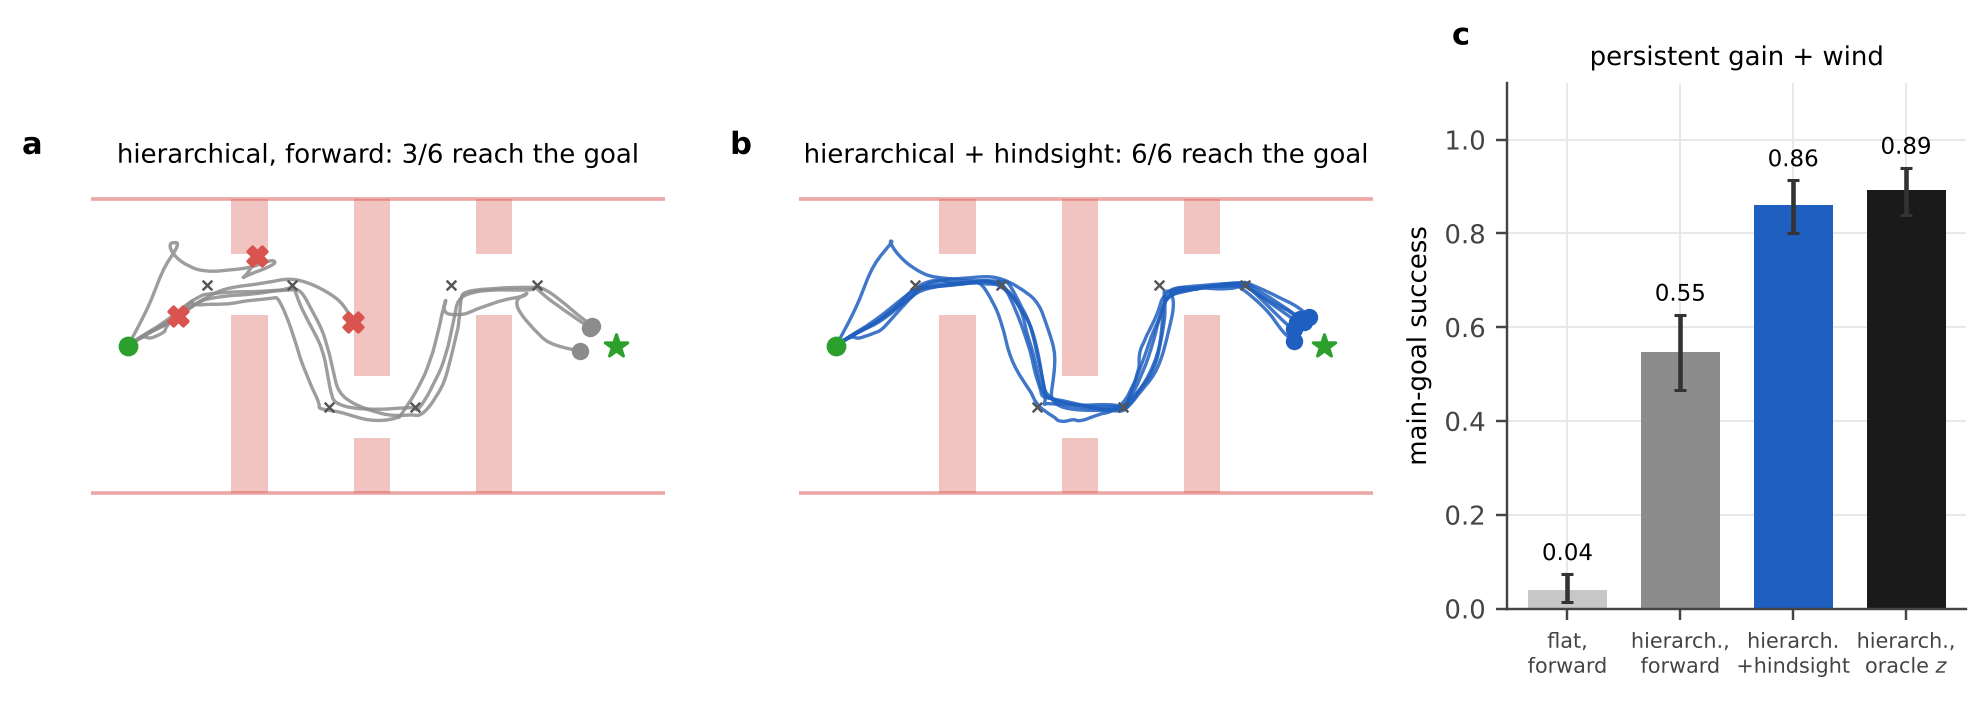
\includegraphics[width=\linewidth]{generated/v7_teaser.png}
\caption{\textbf{Hindsight keeps hierarchical plans alive under a persistent surprise.} A puck must pass three gates in
hazard walls (red; touching one ends the episode) under a hidden motor gain and wind. Both planners use the same learned
world model, the same subgoals (crosses) and the same MPC. (a) Forward planning executes each subgoal as predicted and
drifts into walls. (b) Hindsight infers the latent from the first transitions and stays in the gaps. Six example
episodes with identical latents. (c) Main-goal success over \hiEpisodes{} episodes (95\% bootstrap intervals).}
\label{fig:teaser}
\end{figure}

% ===============================================================================================================
\section{Introduction}

A world model lets an agent plan by imagining the consequences of its actions. Hierarchical world models extend
this to long tasks: a high level proposes subgoals, and a low level reaches them
\citep{lecun2022path,hjepa_2610_06805}. Both levels plan with predictions. When the world contains a factor the model
did not anticipate and that does not go away (a persistent crosswind, a motor weaker than in training, a heavier
object), the predictions are wrong in the same direction every time. The low level misses its subgoal, the high level
replans from wherever the agent ended up, and the next subgoal is missed for the same reason. If a miss is
irreversible (a collision, a fall, a dropped object), the main goal is lost.

Most model-based planners treat each new observation as a fresh starting point. They do not ask why the previous
prediction was wrong. \emph{Hindsight planning} asks exactly that. In the latent-variable formulation of world models
\citep{lecun2022path}, the predictor takes a latent $z$ for what the state and action do not determine. Standard planners
fix $z$ at a nominal value, sample it, or plan against the worst case. When $z$ persists, each executed action is an
experiment about it, and the outcome is evidence that a forward planner discards. Hindsight planning keeps the
predictor frozen, infers $z$ from the agent's own recent history by minimising prediction energy, and plans under the
inferred belief (Figure~\ref{fig:arch}). The hierarchy draws the route; hindsight corrects the model the route is
executed with.

\paragraph{Contributions.}
\begin{enumerate}
\item \textbf{Formulation.} Hindsight planning as posterior inference over the latent of an energy-based world model,
then planning under the posterior. Forward planning, reusing the last residual \citep{cwm_2611_24778} and test-time
latent optimisation \citep{t2z_2610_22364} are the same filter at gains $0$, $1$ and the Bayes gain
(Section~\ref{sec:method}). Hindsight relabeling of achieved outcomes is added as a second, complementary use of the
past.
\item \textbf{Theory} (Section~\ref{sec:theory}). Hindsight is never worse than forward planning; with a persistent latent
its regret is $O(\sigma^2 d\log T)$ against $\Theta(T)$; it gains nothing when the latent is redrawn; residual reuse is
inconsistent; and a hierarchical planner gains exactly when a surprise is identified before failure is irreversible.
\item \textbf{Hierarchical planning with and without hindsight} (Section~\ref{sec:hier}). Hindsight is the difference
between a hierarchical planner that fails half the time and one that nearly matches an oracle, and the size of the
difference follows the theory's conditions.
\item \textbf{Relabeling} (Section~\ref{sec:relabel}). Anchoring predictions on the past outcome closest to the current
goal cancels the world model's local bias, and combined with latent inference it meets an oracle-gap criterion that
latent inference alone failed.
\item \textbf{Mechanisms, realism and real time} (Sections~\ref{sec:mech}--\ref{sec:deploy}). Persistence, commitment
and feedback delay each control the gain; the effect is measured under unmodelled physics, sensor noise, actuation
delay and measured compute delay; and the planner runs in real time.
\item \textbf{Protocol} (Section~\ref{sec:protocol}). Pre-registration, oracle gates, sealed seeds, automated leakage and
causality tests, verified simulator and browser port, and numbers generated only from results files.
\end{enumerate}

\begin{figure}[t]\centering
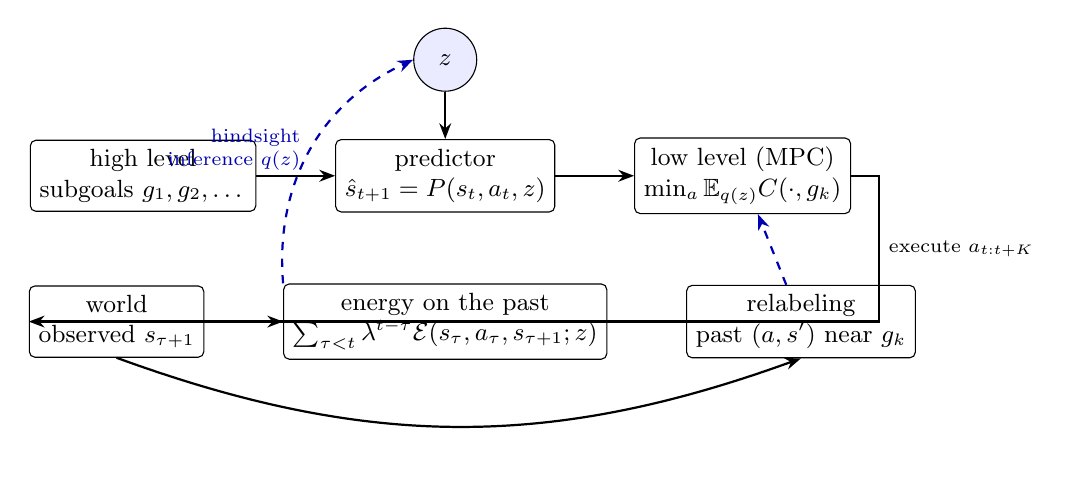
\begin{tikzpicture}[
  box/.style={draw, rounded corners=2pt, minimum height=0.85cm, minimum width=2.1cm, align=center, font=\small},
  lat/.style={draw, circle, minimum size=0.8cm, font=\small, fill=blue!8},
  arr/.style={-{Stealth[length=2mm]}, thick},
  darr/.style={-{Stealth[length=2mm]}, thick, dashed, blue!70!black}]
  \node[box] (hl) {high level\\subgoals $g_1,g_2,\dots$};
  \node[box, right=1.0cm of hl] (pred) {predictor\\$\hat s_{t+1}=P(s_t,a_t,z)$};
  \node[box, right=1.0cm of pred] (actor) {low level (MPC)\\$\min_a \mathbb E_{q(z)}C(\cdot,g_k)$};
  \node[lat, above=0.6cm of pred] (z) {$z$};
  \node[box, below=0.9cm of pred] (energy) {energy on the past\\$\sum_{\tau<t}\lambda^{t-\tau}\E(s_\tau,a_\tau,s_{\tau+1};z)$};
  \node[box, left=1.0cm of energy] (world) {world\\observed $s_{\tau+1}$};
  \node[box, right=1.0cm of energy] (relabel) {relabeling\\past $(a,s')$ near $g_k$};
  \draw[arr] (hl) -- (pred); \draw[arr] (pred) -- (actor); \draw[arr] (z) -- (pred);
  \draw[arr] (world) -- (energy); \draw[arr] (world.south) to[bend right=20] (relabel.south);
  \draw[darr] (energy.north west) to[bend left=35] node[left, font=\scriptsize, align=right]{hindsight\\inference $q(z)$} (z.west);
  \draw[darr] (relabel) -- (actor);
  \draw[arr] (actor.east) -- ++(0.35,0) |- node[pos=0.25, right, font=\scriptsize]{execute $a_{t:t+K}$} (world.west);
\end{tikzpicture}
\caption{Hindsight planning in a hierarchical world model. The high level supplies subgoals. The low level plans with a
frozen predictor whose latent $z$ is inferred from the energy of past predictions (dashed). Relabeling uses past
achieved outcomes as known examples near the current subgoal. Executing $K$ actions open-loop produces new evidence.}
\label{fig:arch}
\end{figure}

% ===============================================================================================================
\section{Hindsight planning}
\label{sec:method}

\paragraph{World model and energy.} A predictor maps state, action and latent to the next state,
$\hat s_{t+1}=P(s_t,a_t,z)$, and scores an observed transition by its energy
$\E(s_t,a_t,s_{t+1};z)=\tfrac12\|s_{t+1}-P(s_t,a_t,z)\|^2_{\Sigma^{-1}}$.

\paragraph{Hindsight inference.} Given the agent's history $\mathcal H_t$, the hindsight posterior is the Gibbs
distribution of the accumulated energy with forgetting $\lambda\le1$,
\begin{equation}
q_t(z)\;\propto\;p(z)\exp\Big(-\textstyle\sum_{\tau<t}\lambda^{\,t-1-\tau}\,\E(s_\tau,a_\tau,s_{\tau+1};z)\Big).
\label{eq:post}
\end{equation}
We use three inference engines: a Gaussian posterior over a multiplicative and an additive correction of the
predicted increment (exact when the correction enters linearly; recursive least squares with forgetting); a particle
posterior with an online estimate of the residual variance; and gradient descent on~\eqref{eq:post}
\citep{t2z_2610_22364}.

\paragraph{Planning under the posterior.} The planner minimises expected cost,
$a^\star_{t:t+H}=\arg\min_a\mathbb E_{z\sim q_t}\big[\sum_k C(\hat s_{t+k}(a,z))\big]$, by the cross-entropy method,
executes the first $K$ actions open-loop, observes, updates $q$, and replans. Forward planning is the same with
$q_t=p$; the oracle uses the true $z$.

\paragraph{One filter, three gains.} For an additive latent following a random walk, the posterior mean is a Kalman
filter on the residual $r_t=s_{t+1}-P(s_t,a_t,\bar z)$. Forward planning has gain $0$; reusing the last residual
\citep{cwm_2611_24778}, equivalently closing the last observed gap between outcome and goal, has gain $1$; for a
persistent latent the Bayes gain decays as $1/t$.

\paragraph{Hindsight relabeling.} Hindsight experience replay treats an outcome the agent actually reached as a goal
it knows how to reach \citep{andrychowicz2017her}. For planning, this gives a second use of the past: among the
executed actions, take the one whose achieved outcome $y^\star$ is closest to the current goal, and predict any action's
outcome as $y^\star+P(a,z)-P(a^\star,z)$. The model then predicts only a difference from a true example in this world,
which cancels its local bias. Combined with inference, $z$ is drawn from $q_t$.

\paragraph{Hindsight in a hierarchy.} All levels share one belief $q_t(z)$, so evidence from one subgoal informs
every later one. In our experiments the high level supplies fixed subgoals and hindsight acts through the shared
belief; redrawing the subgoals themselves is discussed in Section~\ref{sec:lim}.

% ===============================================================================================================
\section{When must hindsight help? Theory}
\label{sec:theory}

Statements and proofs are in Appendix~\ref{sec:theory-full}. Let $z=(\theta,w)$, with a multiplicative part $\theta$
(it scales the effect of an action) and an additive part $w$, $d=2$, and observation noise $\sigma^2$.
\begin{enumerate}
\item \textbf{Dominance} (Thm.~\ref{thm:dominance}): the Bayes hindsight planner is never worse than any forward
planner \citep{blackwell1953}.
\item \textbf{Persistence is necessary} (Thm.~\ref{thm:fresh}): if $z$ is redrawn every step, the posterior predictive
equals the prior and hindsight gains nothing; a planner that assumes persistence can lose.
\item \textbf{Persistence suffices for a large gain} (Thm.~\ref{thm:separation}): forward regret is $\Theta(T)$,
hindsight regret $O(\sigma^2d\log T)$, with per-step excess $\sigma^2d/t$.
\item \textbf{Last-residual reuse is inconsistent} (Thm.~\ref{thm:residual}): it pays $\sigma^2$ per step forever under
an additive $z$, is unstable when $\theta>2\bar\theta$, and is worse than forward planning with no disturbance.
\item \textbf{Hierarchy} (Thm.~\ref{thm:hier}): under a persistent $z$, a hierarchical planner whose subgoal execution
ignores outcomes fails with the same probability on every retry; hindsight's advantage is the probability that a
subgoal is infeasible under the nominal model \emph{and} the surprise is identified before failure is irreversible.
\end{enumerate}
The theory names three conditions for a large gain: the latent persists; the planner commits to actions before
feedback can correct them (open-loop execution, one-shot decisions, observation delay); and the data excite the
latent enough to identify it. Sections~\ref{sec:hier}--\ref{sec:mech} vary each one.

% ===============================================================================================================
\section{Protocol}
\label{sec:protocol}
\textbf{Pre-registration.} Each experiment's hypotheses, planners, seeds, sample sizes and decision rules, and the
script that applies them, were committed before the run; outcomes, including failures, are appended to the same file.
\textbf{Oracle gates.} Before a new task is used, the planner given the true latent must beat forward planning by a
declared margin; task parameters may only be chosen from a declared ladder using forward and oracle results.
\textbf{Data separation.} World models are trained on random-action data that contains no task, goal or test
latent; test latents, goals, planner randomness, gates and the sealed deployment test use pairwise disjoint seed
streams. \textbf{Leakage and causality tests.} Automated tests check that no non-oracle planner's actions change when
the true latent is replaced by garbage (and that the oracle's do), that trajectories in two worlds identical up to step
$t^\star$ are identical up to $t^\star$ (with noise and delays on), and that every realism option takes effect.
\textbf{Verification.} The simulator matches closed-form dynamics to $10^{-9}$ with perturbed mass and damping (this test
caught a mass change that MuJoCo silently ignored before any affected run); the browser port matches the Python and
MuJoCo code to between $10^{-16}$ and $10^{-7}$. \textbf{Statistics.} All planners face the same episodes; intervals are
95\% paired bootstrap over episodes. \textbf{Provenance.} Results carry the git commit and a clean-tree flag recorded
before the run; every number in this paper is generated from them. The full protocol is in \texttt{EVALUATION.md}.

% ===============================================================================================================
\section{Hierarchical planning with and without hindsight}
\label{sec:hier}

\paragraph{Task.} A puck driven by two motors (MuJoCo \citep{todorov2012mujoco}) must travel from $(0,0)$ to $(4,0)$
through gaps of width 0.5\,m in three hazard walls (Figure~\ref{fig:teaser}); touching a wall or the arena boundary
ends the episode. The hidden latent is the motor gain ($U[0.4,1.6]$) and a constant wind ($\mathcal N(0,1)$\,N per
axis). Regimes: no latent, persistent wind, persistent gain and wind, and a \emph{fresh} control in which both are
redrawn every second. \textbf{Planners.} A \emph{flat} planner plans directly to the goal. A \emph{hierarchical}
planner receives subgoals (the approach and exit point of each gap, then the goal) and reaches each with CEM-MPC on a
learned five-member ensemble world model (horizon 15 steps, hazard penalty in the rollout), executing open-loop chunks
of $K=10$ steps (0.5\,s). We compare the hierarchical planner with forward planning, last-residual reuse, online
fine-tuning of the model's last layer \citep{adajepa_2606_32026}, hindsight with the Gaussian posterior, hindsight with
particles, and the oracle. \hiEpisodes{} episodes per cell (3 seeds of models $\times$ 50), same episodes for every
planner. The oracle gate passed at the first gap width on the pre-declared ladder.

\begin{table}[t]\centering\small
\begin{tabular}{lcccc}
\toprule
Planner & no latent & persistent wind & persistent gain + wind & fresh \\
\midrule
flat, forward & 0.41 & 0.09 & 0.04 & 0.01 \\
flat, hindsight & 0.00 & 0.00 & 0.00 & 0.00 \\
hier., forward & 1.00 & 0.73 & 0.55 & 0.36 \\
hier. + residual & 1.00 & 0.95$^{+}$ & 0.77$^{+}$ & 0.39 \\
hier. + online SGD & 1.00 & 0.84$^{+}$ & 0.64$^{+}$ & 0.37 \\
hier. + hindsight & 1.00 & 0.94$^{+}$ & 0.86$^{+}$ & 0.25$^{-}$ \\
hier. + hindsight (particles) & 1.00 & 0.95$^{+}$ & 0.83$^{+}$ & 0.37 \\
hier., oracle $z$ & 1.00 & 0.98$^{+}$ & 0.89$^{+}$ & 0.94$^{+}$ \\
\bottomrule
\end{tabular}

\caption{Main-goal success. $^{+}$/$^{-}$: 95\% paired interval of the difference to hierarchical forward planning
entirely above/below zero.}
\label{tab:hier}
\end{table}

\begin{figure}[t]\centering
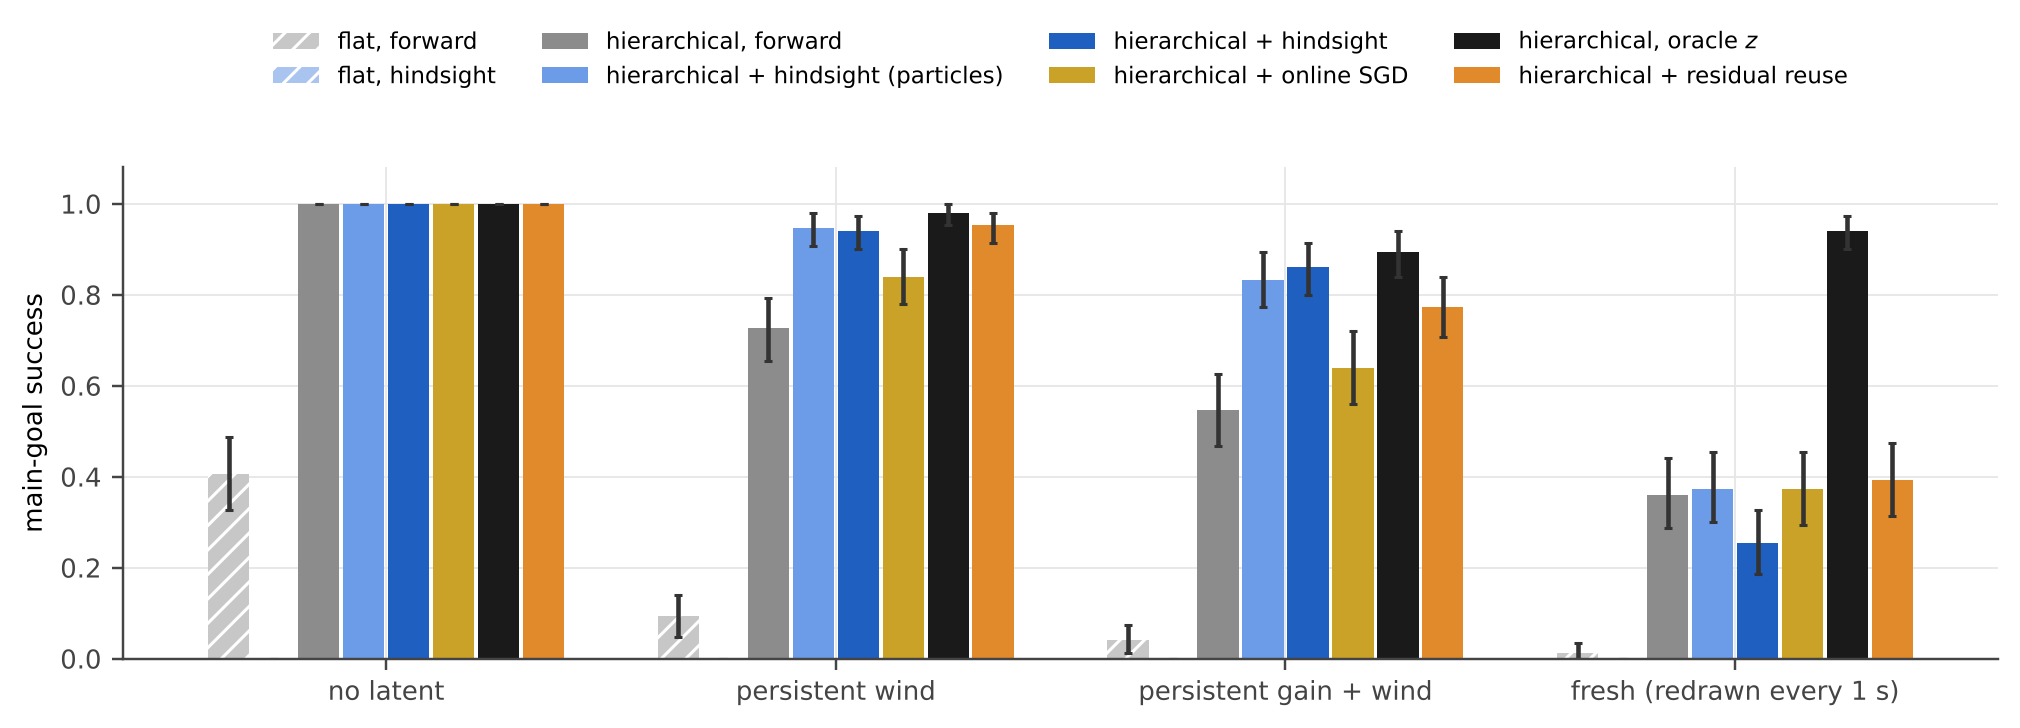
\includegraphics[width=\linewidth]{generated/v7_success.png}
\caption{Main-goal success by latent regime (95\% bootstrap intervals; hatched: flat planners).}
\label{fig:hier}
\end{figure}

\paragraph{Results (Table~\ref{tab:hier}, Figure~\ref{fig:hier}).} All seven pre-registered predictions held.
\emph{Hierarchy is needed:} with no latent, every hierarchical planner succeeds in every episode, flat forward planning in
\hiFlatNone{} of them. \emph{Hierarchy alone is not enough:} under a persistent gain and wind, hierarchical forward
planning succeeds in \hiFwdBoth{} of episodes. \emph{Hindsight closes most of the gap:} the same hierarchical planner with
hindsight succeeds in \hiHindBoth{} (difference \hiDiffBoth, interval [\hiDiffLoBoth, \hiDiffHiBoth]); the oracle reaches
\hiOracleBoth, so hindsight recovers \hiCapture{} of the improvement available. Under wind alone the numbers are
\hiFwdWind{}, \hiHindWind{} and \hiOracleWind. \emph{Inference beats cheaper corrections where the latent is
multiplicative:} residual reuse reaches \hiResidBoth{} and online fine-tuning \hiSgdBoth{} under gain and wind; under
wind alone residual reuse matches hindsight (\hiResidWind), as expected for an additive latent. \emph{Controls:} with
no latent hindsight changes nothing; with a latent redrawn every second it is worse than forward planning (\hiHindFresh{}
vs \hiFwdFresh), as Theorem~\ref{thm:fresh} requires.

\begin{figure}[t]\centering
\begin{minipage}{0.64\linewidth}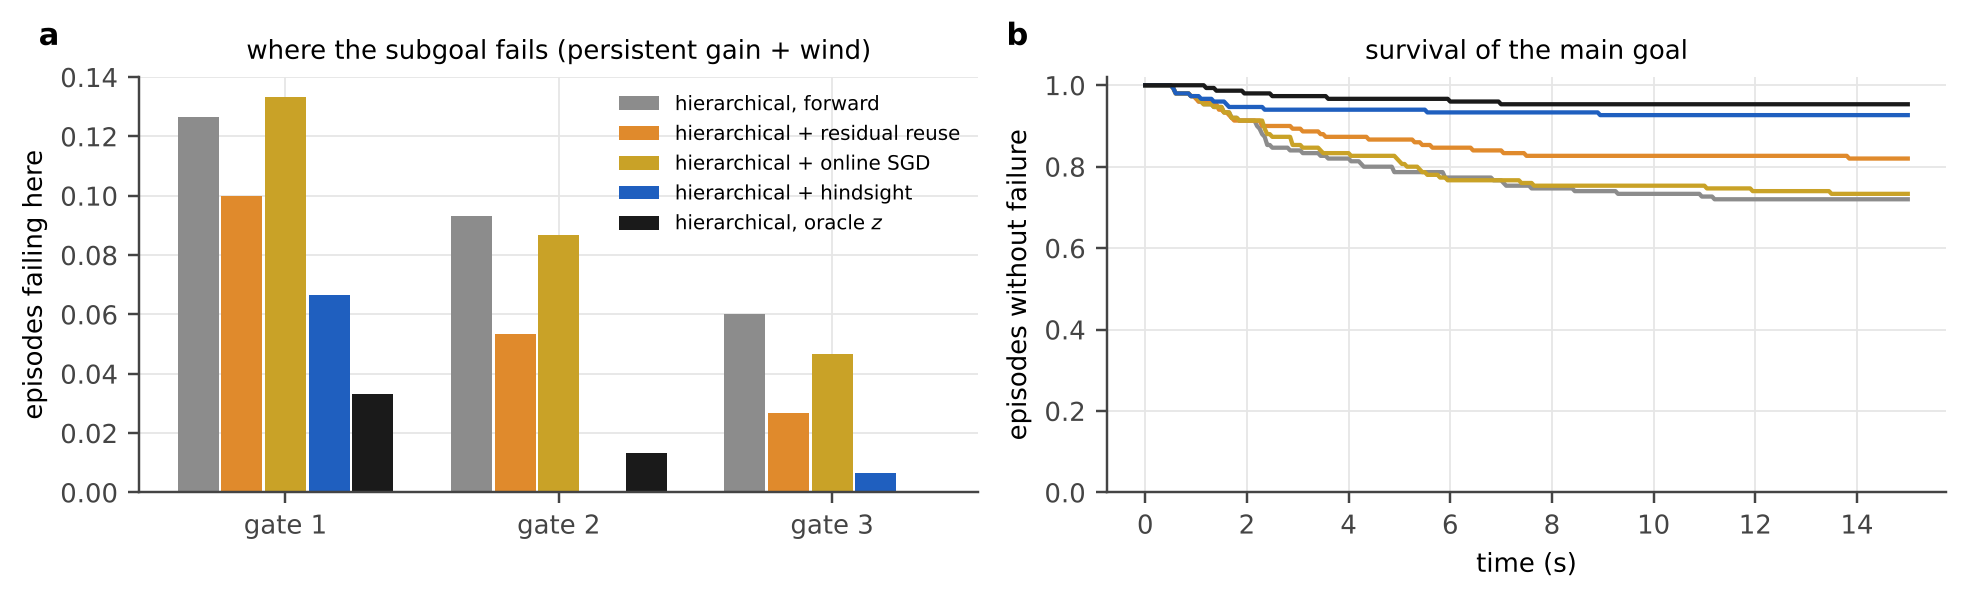
\includegraphics[width=\linewidth]{generated/v7_failures.png}\end{minipage}\hfill
\begin{minipage}{0.34\linewidth}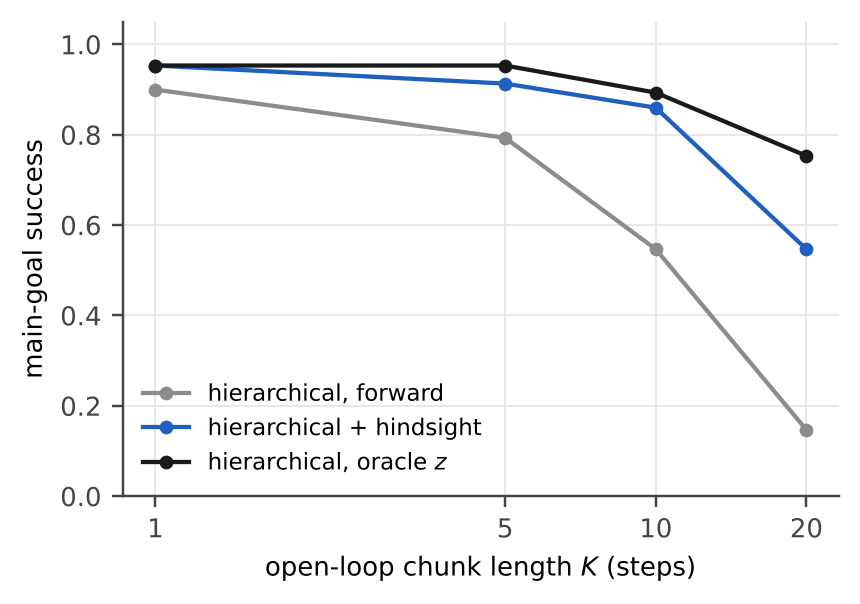
\includegraphics[width=\linewidth]{generated/v7_ksweep.png}\end{minipage}
\caption{Left: where the main goal is lost under a persistent gain and wind (a) and the fraction of episodes without a
failure over time (b). Forward planning loses episodes at every gate; hindsight loses a few at the first gate, while it
is still identifying the latent, and almost none afterwards. Right: success against the open-loop chunk length $K$.}
\label{fig:fail}
\end{figure}

\paragraph{Subgoal failure.} Figure~\ref{fig:fail}a shows the mechanism of Theorem~\ref{thm:hier}. Forward planning
fails at every gate because the same unmodelled latent defeats every subgoal. Hindsight's failures concentrate at the
first gate, before the latent has been identified, and almost vanish afterwards.

\paragraph{Commitment.} Fast replanning absorbs much of a disturbance; committing to longer open-loop segments does not
(Figure~\ref{fig:fail}, right). Hindsight's gain in success over forward planning grows monotonically with the chunk
length: \hkGainOne{} at $K=1$, \hkGainFive{} at $K=5$, \hkGainTen{} at $K=10$ and \hkGainTwenty{} at $K=20$.

\paragraph{Hindsight does not replace hierarchy, and can hurt a flat planner.} A flat planner with hindsight
succeeded in no episode in any regime, including the one without a latent. Diagnosis (not pre-registered): failures
are head-on collisions with the first wall at in-distribution speeds; with no latent at all the posterior acquires a
spurious offset (about $-0.5$\,N), absorbing the world model's own bias, and the planner then predicts that it stops
short of the wall while it does not. Subgoals placed in the open gap row protect the hierarchical planner from this.
Hindsight inference can absorb model bias into the latent and hurt plans that depend on exact stopping distances near
hazards.

% ===============================================================================================================
\section{Relabeling: anchoring the plan on what actually happened}
\label{sec:relabel}

\paragraph{Task.} A puck is launched with a chosen velocity at a target and flies for 2\,s under a hidden damping
($U[0.5,2]$) and wind ($\mathcal N(0,0.5^2)$\,N per axis). Each episode has \twAttempts{} throws at new random targets
under the same latent; every throw is a one-shot open-loop decision. \twEpisodes{} episodes. Regimes: wind only
(additive), damping only (multiplicative), both, and fresh (redrawn every throw).

\paragraph{Planners.} \emph{Goal-gap correction} aims so that predicted outcome plus a correction equals the target, and
adds each throw's outcome-minus-target gap to the correction (an integral controller on the gap). \emph{Mean gap} uses
the mean of past model errors. \emph{Relabeling anchor} predicts from the past throw whose landing point is closest to
the current target (Section~\ref{sec:method}). \emph{Latent inference} is the particle posterior with
posterior-expected cost. \emph{Latent inference + relabeling} applies the anchor under each posterior sample.

\begin{table}[t]\centering\small
\begin{tabular}{lcccc}
\toprule
Planner & wind & damping & both & fresh \\
\midrule
goal-gap correction & 0.187 & 0.634 & 0.414 & 1.416 \\
residual reuse & 0.180 & 0.603 & 0.391 & 1.407 \\
mean gap & 0.147 & 0.477 & 0.321 & 1.143 \\
relabeling anchor & 0.113 & 0.379 & 0.269 & 1.326 \\
latent inference & 0.189 & 0.321 & 0.238 & 1.269 \\
latent inference + relabeling & 0.096 & 0.209 & 0.169 & 1.341 \\
oracle $z$ & 0.030 & 0.138 & 0.125 & 0.107 \\
\midrule
final-attempt miss / oracle, latent inference & 6.0 & 2.2 & 1.8 & -- \\
final-attempt miss / oracle, + relabeling & 1.8 & 1.1 & 1.1 & -- \\
\bottomrule
\end{tabular}

\caption{Repeated throwing: mean miss over attempts 2--\twAttempts{} relative to forward planning (lower is better;
all intervals in \texttt{generated/v9\_summary.txt}), and final-attempt miss relative to the oracle.}
\label{tab:v9}
\end{table}

\begin{figure}[t]\centering
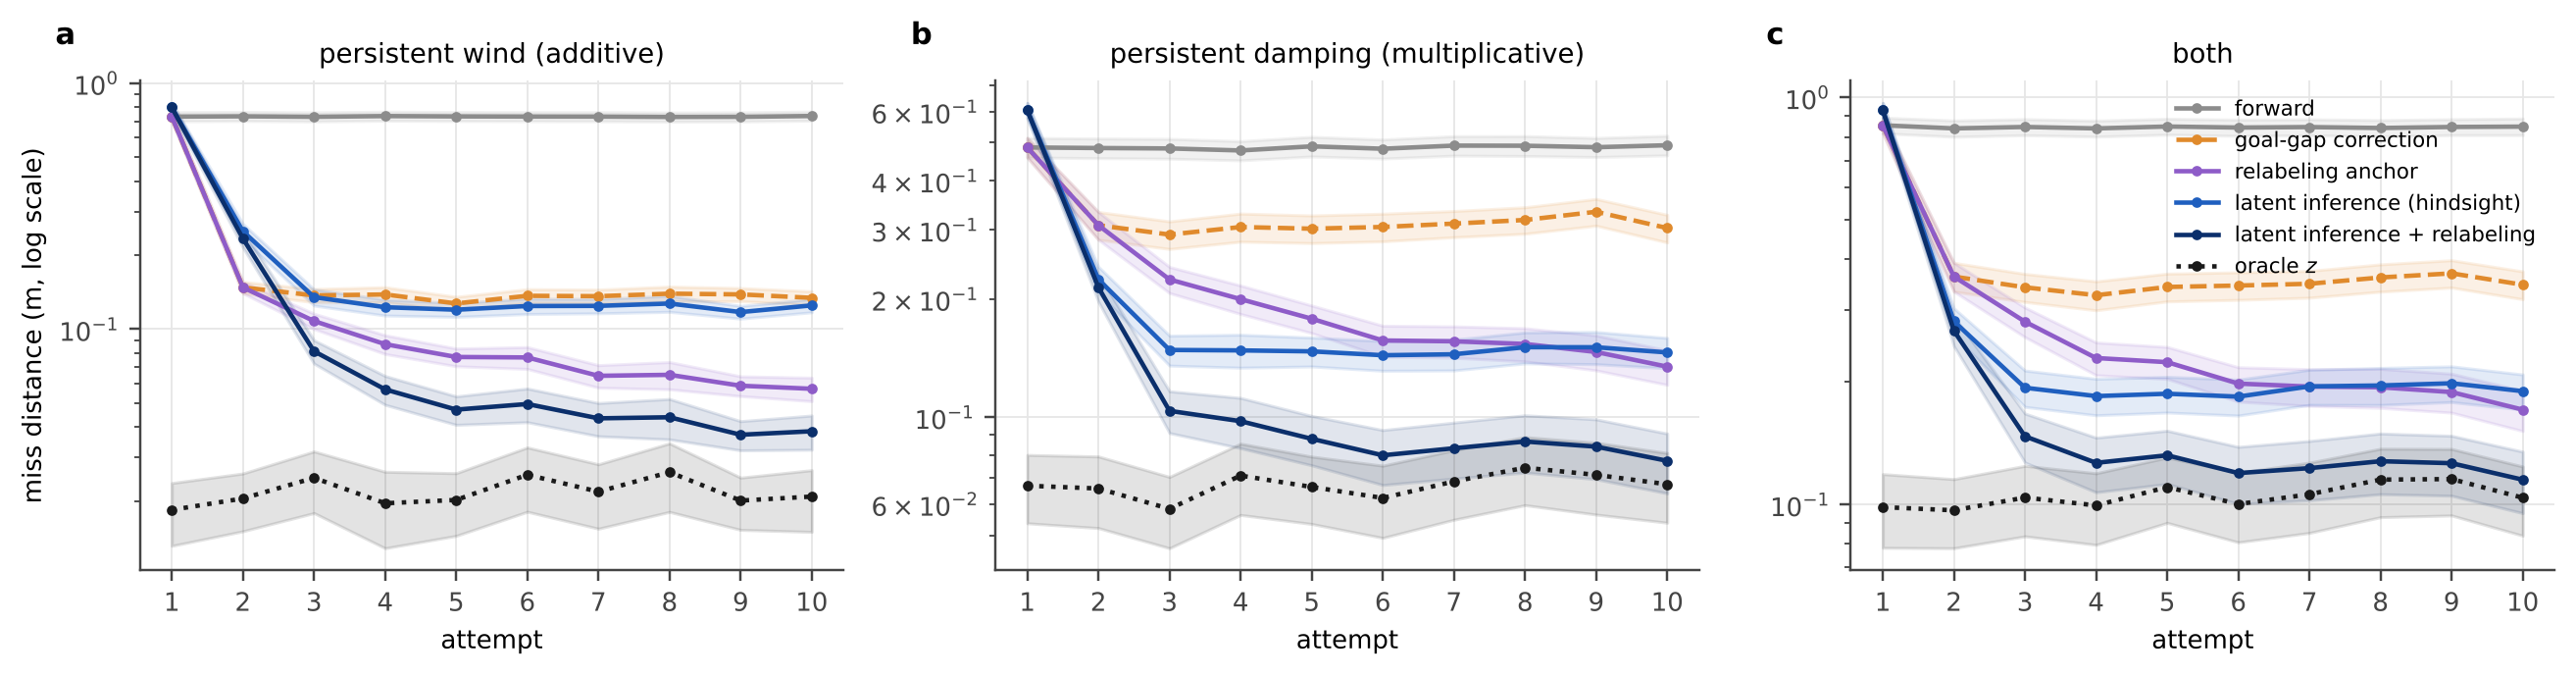
\includegraphics[width=\linewidth]{generated/v9_figure.png}
\caption{Miss distance per attempt (log scale, $\pm2$ s.e.). Forward planning never improves. Goal-gap correction
learns an additive offset in one throw but cannot represent damping. Latent inference with relabeling approaches the
oracle.}
\label{fig:v9}
\end{figure}

\paragraph{Results (Table~\ref{tab:v9}, Figure~\ref{fig:v9}).} All pre-registered predictions held. Goal-gap correction
behaves like last-residual reuse, as the theory predicts: it reduces the miss to \vnGapWind{} of forward planning under
wind, but only to \vnGapDamp{} under damping, because the gap left by one throw does not transfer to a throw at a
different target when the latent scales the action's effect. Relabeling beats it wherever the latent is multiplicative
(\vnAnchorDamp{} under damping). Latent inference with relabeling is the best non-oracle planner in every persistent
regime (\vnHAWind, \vnHADamp, \vnHABoth{} for wind, damping and both), reducing the miss left by latent inference alone
by \vnHAvsHWind, \vnHAvsHDamp{} and \vnHAvsHBoth. Its final throw misses by \vnHAOracleWind, \vnHAOracleDamp{} and
\vnHAOracleBoth{} times the oracle's distance, against \twOracleGapWind, \twOracleGapDamp{} and \twOracleGapBoth{} for latent
inference alone; the pre-registered criterion of at most twice the oracle, failed by inference alone, is met in all
three regimes. When the latent is redrawn every throw, every method that uses the past is worse than forward planning
(for example \vnHAFresh).

% ===============================================================================================================
\section{What controls the gain}
\label{sec:mech}
Each condition of the theory was varied with everything else fixed, in a puck-navigation task with learned models and
CEM-MPC (cost relative to forward planning; lower is better).

\paragraph{Persistence.} With AR(1) wind of persistence $\rho$, the particle posterior's cost ratio falls monotonically
from \rhoZero{} at $\rho=0$ (worse than forward) to \rhoOne{} at $\rho=1$ (Table~\ref{tab:rho}).

\paragraph{Commitment.} With replanning every step, hindsight's gain is \ksGainOne; with open-loop chunks of 40 steps it
is \ksGainForty{} against an oracle headroom of \ksHeadForty{} (Table~\ref{tab:k}).

\paragraph{Feedback delay.} When observations arrive $d$ steps late, every planner reconstructs the present by rolling
its own believed model forward, so hindsight improves both the plan and the state estimate. Its gain grows from
\dlGainZero{} at $d=0$ to \dlGainTwenty{} at $d=20$, while online fine-tuning reaches \dlSgdTwenty{} of forward cost at
$d=20$ against \dlPostTwenty{} for hindsight (Table~\ref{tab:delay}, Figure~\ref{fig:v6}c).

\paragraph{One-shot decisions.} In repeated throwing (Section~\ref{sec:relabel}) the miss of latent inference alone is
\twHindBoth{} of forward planning; when the latent is redrawn every throw it is \twHindFresh{} (Figure~\ref{fig:v6}a,b).

\paragraph{Noise and calibration.} With i.i.d.\ gusts added to a persistent wind, last-residual reuse degrades from
\nzResidZero{} to \nzResidOne{} while the Gaussian posterior stays at \nzPostZero{}--\nzPostOne{}. A particle posterior
whose likelihood width is fixed from training residuals chases the gusts (\nzFixedZero{} $\to$ \nzFixedOne); estimating
the residual variance online restores it (\nzAdaptZero{} $\to$ \nzAdaptOne) (Table~\ref{tab:noise}).

\begin{table}[t]\centering\scriptsize
\begin{minipage}{0.49\linewidth}\centering\begin{tabular}{lccccc}
\toprule
$K$ & 1 & 5 & 10 & 20 & 40 \\
\midrule
hindsight gain (wind) & 0.4\% & 0.3\% & 4.3\% & 17.9\% & 34.1\% \\
oracle headroom (wind) & 0.7\% & 1.9\% & 7.7\% & 29.2\% & 49.1\% \\
hindsight gain (both) & 0.8\% & 1.4\% & 5.9\% & 22.6\% & 35.6\% \\
oracle headroom (both) & 1.5\% & 2.5\% & 9.1\% & 35.2\% & 52.0\% \\
\bottomrule
\end{tabular}
\captionof{table}{Gain over forward by chunk length.}\label{tab:k}\end{minipage}\hfill
\begin{minipage}{0.49\linewidth}\centering\begin{tabular}{lcccc}
\toprule
$\rho$ & 0.0 & 0.9 & 0.99 & 1.0 \\
\midrule
latent (particles) & 1.221 & 1.058 & 0.840 & 0.736 \\
posterior & 1.018 & 1.015 & 0.819 & 0.707 \\
residual reuse & 1.311 & 0.993 & 0.764 & 0.703 \\
oracle & 1.216 & 0.936 & 0.685 & 0.586 \\
\bottomrule
\end{tabular}
\captionof{table}{Cost ratio by persistence $\rho$.}\label{tab:rho}\end{minipage}
\vspace{0.5em}

\begin{minipage}{0.49\linewidth}\centering\begin{tabular}{lcccc}
\toprule
delay (steps) & 0 & 5 & 10 & 20 \\
\midrule
hindsight (posterior) & 0.977 & 0.901 & 0.756 & 0.633 \\
hindsight (particles) & 0.984 & 0.915 & 0.768 & 0.639 \\
online SGD & 0.986 & 0.948 & 0.891 & 0.876 \\
oracle & 0.975 & 0.882 & 0.692 & 0.447 \\
\bottomrule
\end{tabular}
\captionof{table}{Cost ratio by observation delay.}\label{tab:delay}\end{minipage}\hfill
\begin{minipage}{0.49\linewidth}\centering\begin{tabular}{lcccc}
\toprule
gust sd (N) & 0.0 & 0.25 & 0.5 & 1.0 \\
\midrule
posterior & 0.790 & 0.792 & 0.794 & 0.803 \\
latent, adaptive likelihood & 0.793 & 0.797 & 0.810 & 0.840 \\
latent, fixed likelihood & 0.821 & 0.865 & 0.912 & 1.001 \\
residual reuse & 0.783 & 0.795 & 0.833 & 0.981 \\
oracle & 0.708 & 0.710 & 0.712 & 0.716 \\
\bottomrule
\end{tabular}
\captionof{table}{Cost ratio under gust noise.}\label{tab:noise}\end{minipage}
\end{table}

\begin{figure}[t]\centering
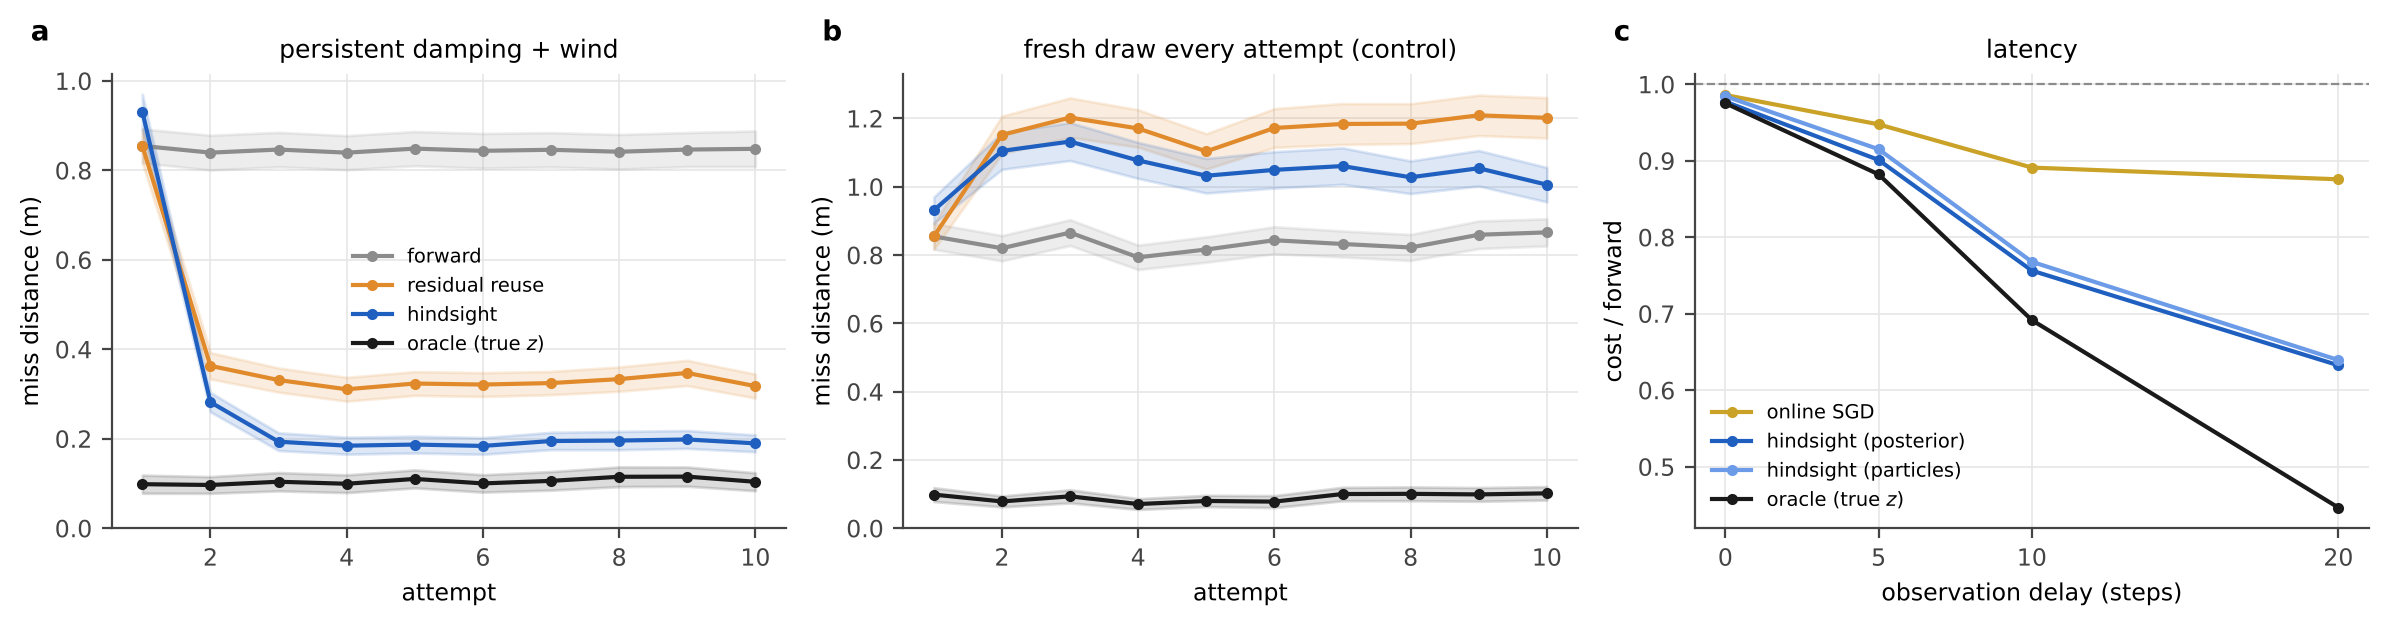
\includegraphics[width=\linewidth]{generated/v6_figure.png}
\caption{(a) Repeated throwing under persistent damping and wind; (b) the same with the latent redrawn every throw;
(c) cost relative to forward planning as observation delay grows.}
\label{fig:v6}
\end{figure}

\paragraph{What the inferred latent represents.}\label{sec:ident}\label{sec:probe} A linear probe from the posterior to the
true latent explains \idWindTwenty{} of the wind's variance after 20 transitions, while the motor gain is poorly
identified and the inferred parameters dip at every chunk boundary. The data constrain $\theta a+w$, not $\theta$ and
$w$ separately, and each new action rotates that ridge: pinning the gain removes the dip (\cfDipStd{} $\to$ \cfDipPin), and
the identifiable quantity, the predicted effect of the next action, reaches $R^2=$\idPredEnd. Interpretability claims
about inferred latents should be made about identifiable combinations.

\paragraph{Real measured systems.} On five system-identification benchmarks with official splits
\citep{nonlinear_benchmarks}, where inputs are logged and no planner acts, the Gaussian posterior reduces ten-step
prediction error to \rdTenStep{} of the frozen model's while last-residual reuse increases it to \rdResidTen; online
fine-tuning is stronger here (\rdSgdFwdTen), and adding the posterior to it gives no further gain (\rdHybridSgd).

% ===============================================================================================================
\section{Deployment realism and real time}
\label{sec:deploy}

Every result above assumes perfect sensing, instant actuation, free compute, and deployment physics that differ from
training only through the latent. A deployed controller has none of these. We re-ran the hierarchical task on three
\emph{sealed} seeds, never used for any design decision, with four realism factors fixed in advance:
\textbf{unmodelled physics} (mass $\times U[0.8,1.25]$ and damping $\times U[0.7,1.4]$ per episode, which the world model never
saw and which the oracle is not told); \textbf{sensor noise} (1\,cm on position, 5\,cm/s on velocity, on everything the
planner sees); \textbf{actuation delay} of one control step (50\,ms); and \textbf{measured compute delay}. For the last,
each planner's 95th-percentile decision time for one robot on one CPU thread was measured once on an idle machine and
converted into control steps (\dpStepsHind{} for hindsight, \dpStepsFwd{} for forward planning); while a decision is being
computed the robot keeps executing its previous plan, so a slower planner pays for its compute. Hazards and success are
judged on the true state.

\begin{table}[t]\centering\small
\begin{tabular}{lcccc}
\toprule
Planner & idealised & deployment & deployment, no latent & deployment, fresh \\
\midrule
hier., forward & 0.55 & 0.05 & 0.98 & 0.03 \\
hier. + residual & 0.77 & 0.00 & 0.00 & 0.00 \\
hier. + online SGD & 0.64 & 0.15 & 1.00 & 0.03 \\
hier. + hindsight & 0.86 & 0.41 & 0.99 & 0.03 \\
hier. + hindsight (particles) & 0.83 & 0.37 & 0.91 & 0.06 \\
hier., oracle $z$ & 0.89 & 0.72 & 0.98 & 0.76 \\
\bottomrule
\end{tabular}

\caption{Main-goal success under deployment realism (sealed seeds, \dpEpisodes{} episodes per cell). ``Idealised'' is the
persistent gain and wind regime of Table~\ref{tab:hier}; the deployment columns add unmodelled physics, sensor noise,
actuation delay and measured compute delay.}
\label{tab:v8}
\end{table}

\begin{figure}[t]\centering
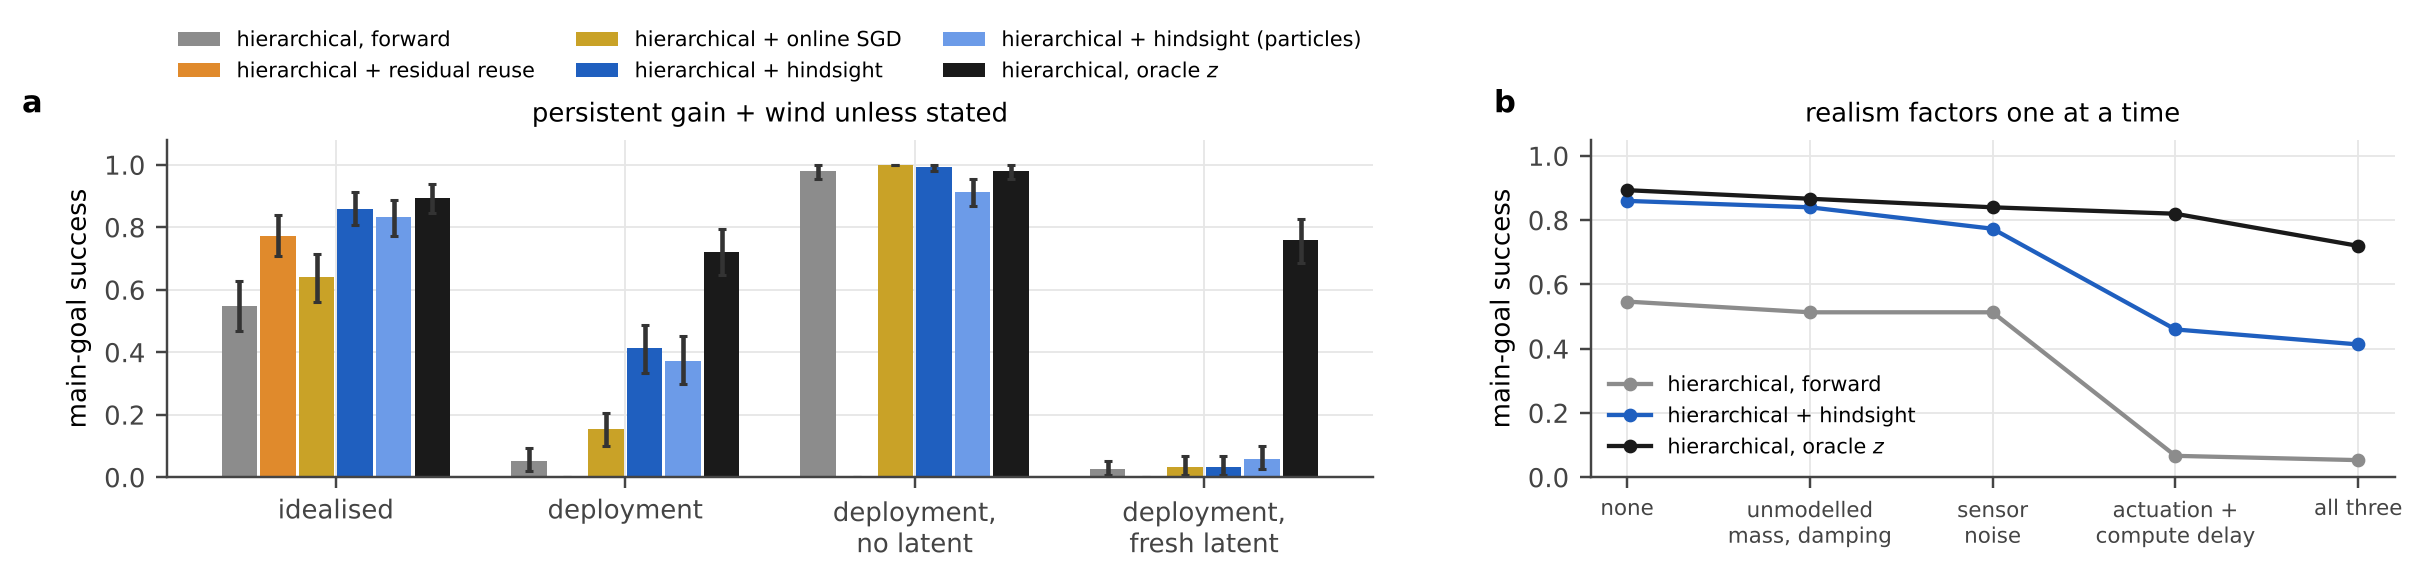
\includegraphics[width=\linewidth]{generated/v8_figure.png}
\caption{(a) Success under deployment realism. (b) The realism factors one at a time (persistent gain and wind):
delay, not noise or unmodelled physics, is what defeats forward planning.}
\label{fig:v8}
\end{figure}

\paragraph{Results (Table~\ref{tab:v8}, Figure~\ref{fig:v8}).} All six pre-registered predictions held. Realism lowers
every planner's success, and the drop is uneven. Under a persistent gain and wind, hierarchical forward planning nearly
collapses (\dpFwdBoth), while the same planner with hindsight keeps \dpHindBoth{} (difference \dpDiffBoth, interval
[\dpDiffLoBoth, \dpDiffHiBoth]); the particle posterior, which pays the same compute delay, reaches \dpPfBoth. The gain
over forward planning is \dpGainRatio{} times its idealised size, but the absolute level is lower: hindsight recovers
\dpCapture{} of the oracle's headroom here, against \hiCapture{} in the idealised task. Taken one at a time, unmodelled
physics and sensor noise cost forward planning little (\abFwdMismatch{} and \abFwdNoise) and hindsight little
(\abHindMismatch{} and \abHindNoise); delay is what matters, cutting forward planning to \abFwdDelay{} while hindsight
keeps \abHindDelay. This is the commitment condition again: delay commits the robot to actions chosen on stale
information, and a correct model of the world is what lets it act well on stale information.

\paragraph{Controls.} With no latent, the Gaussian posterior is indistinguishable from forward planning (\dpHindNone{}
vs \dpFwdNone), but the particle posterior costs success (\dpPfNone; difference \dpPfDiffNone). With a latent redrawn
every second, every non-oracle planner fails (forward \dpFwdFresh, hindsight \dpHindFresh). Last-residual reuse, which
was competitive in the idealised task, fails in every deployment condition including the one with no latent
(\dpResidNone): under sensor noise it chases the noise, as Theorem~\ref{thm:residual} predicts.

\begin{table}[t]\centering\small
\begin{tabular}{lccc}
\toprule
Planner & decision p50 (ms) & decision p95 (ms) & belief update p95 (ms) \\
\midrule
forward & 48 & 51 & 0.06 \\
residual reuse & 49 & 52 & 0.35 \\
online SGD & 48 & 57 & 0.85 \\
hindsight (posterior) & 73 & 79 & 0.68 \\
hindsight (particles) & 54 & 57 & 1.37 \\
oracle & 48 & 49 & 0.05 \\
\bottomrule
\end{tabular}

\caption{Decision and belief-update latency for one robot, one CPU thread (\latCPU), production configuration
(300 candidate plans, 3 CEM iterations, horizon 15, five-member ensemble).}
\label{tab:latency}
\end{table}

\paragraph{Real time.} A decision with the Gaussian posterior takes \latPostOne\,ms at the 95th percentile on one thread
(Table~\ref{tab:latency}), against \latFwdOne\,ms for forward planning; the belief update takes \latObsPost\,ms. With
open-loop chunks of 0.5\,s, planning fits within the budget with room to spare. An interactive version of the task runs
the same seed-0 models and planners in a web browser against a 20\,Hz control clock, with planning in background threads
so that compute latency acts in real time (\texttt{demo/}); its physics, network outputs, belief update and plan costs
match the Python and MuJoCo implementation to between $10^{-16}$ and $10^{-7}$. That browser implementation is
unoptimised and slower than the Python one at the paper's population size.


% ===============================================================================================================
\section{Limitations and negative results}
\label{sec:lim}
\textbf{Privileged training.} The world models are trained with the latent as an input, so the latent space is given,
not learned; in a self-supervised world model \citep{lecun2022path,hjepa_2610_06805} it would have to be discovered, and its
identifiability (Section~\ref{sec:ident}) becomes central. \textbf{Subgoals are not redrawn.} Hindsight acts through the
shared belief; the high level does not change the subgoals. In an earlier river-crossing task designed to need subgoal
redrawing (choosing between fording and a bridge), three pre-registered designs found no benefit (success \rvOneHind{} vs
\rvOneFwd{}; \rvTwoHind{} vs \rvTwoFwd; and a design in which forward planning pushed through, \rvThreeFwd{}, while the
oracle's bridge execution succeeded only \rvThreeOracle{} of the time). Execution and fast feedback decided those
outcomes, not inference. \textbf{Bias absorption.} The flat-planner result of Section~\ref{sec:hier} shows that an
inferred latent can absorb model bias and mislead a planner. \textbf{Oracle gap.} Latent inference alone does not reach
the oracle; relabeling closes much of the gap in the throwing task but was not tested in navigation. \textbf{Scale.}
Low-dimensional state, small MLP ensembles, one simulator and five real benchmarks with logged inputs; no pixels and no
physical robot. \textbf{Excitation.} Multiplicative latents are identified only through variation in the actions;
no planner here explores on purpose.

\section{Related work}
Latent-variable and energy-based world models and hierarchical planning \citep{lecun2022path,hjepa_2610_06805};
test-time adaptation of world models by latent optimisation \citep{t2z_2610_22364} or weight updates
\citep{adajepa_2606_32026,jepattt_2610_00722}; residual reuse in counterfactual world models \citep{cwm_2611_24778};
hindsight experience replay \citep{andrychowicz2017her}; probabilistic ensembles for MPC \citep{chua2018pets}; adaptive
control and regret \citep{laiwei1982,abbasi2011,simchowitz2020,cassel2020,astrom_wittenmark}; value of information
\citep{blackwell1953}; probing world models \citep{li2023othello,probing_rl_wm_2603_21546}.

\section{Discussion}
A hierarchical world model draws the route; it does not know the world it will drive in. Our results suggest a division
of labour: the predictor models what is the same across worlds, a low-dimensional latent carries what is constant within
one, and the agent infers that latent from its own recent history rather than marginalising it away at every step.
Relabeling adds a second, model-light use of the same history, and the two combine. The gains appear where the theory
says they must (persistent surprises, committed actions, delayed feedback) and vanish or reverse where it says they
cannot. Three steps remain before this is a robot result: a latent learned without labels, a high level that redraws
subgoals from the posterior, and a physical system.

\bibliographystyle{plainnat}
\bibliography{../refs}

\appendix
\section{Theory: statements and proofs}
\label{sec:theory-full}
% Body of the theory appendix (generated from theory.tex without its section header).

\paragraph{Setting.} At step $t$ the agent receives a commanded displacement $\delta_t$ (i.i.d., independent of
the past) and chooses a bounded command $|a_t|\le A$. The world responds
\begin{equation}
\Delta s_t=\theta_t a_t+w_t+\varepsilon_t,\qquad \varepsilon_t\sim\mathcal N(0,\sigma^2)\ \text{i.i.d.},
\end{equation}
with cost $c_t=(\Delta s_t-\delta_t)^2$. The hidden disturbance $\phi_t=(\theta_t,w_t)$ has a \emph{gain} part
$\theta_t$ (it scales the command) and an \emph{additive} part $w_t$; its prior is $\mathcal N(m_0,S_0)$ with
$m_0=(\bar\theta,0)$. Let $\mathcal F_t$ be the history $(\delta_{0:t},a_{0:t-1},\Delta s_{0:t-1})$.
A \textbf{forward} planner chooses $a_t$ as a function of $\delta_t$ only (it never conditions on outcomes);
a \textbf{hindsight} planner chooses $a_t$ as a function of $\mathcal F_t$. Regret is measured against the
oracle that knows $\phi_t$ and obeys the same bound; $\varepsilon_t$ is common to all planners and cancels.

\begin{theorem}[Dominance]\label{thm:dominance}
For any prior and any disturbance process, the myopic Bayes hindsight planner
$a^H_t=\arg\min_{|a|\le A}\mathbb E[c_t\mid\mathcal F_t]$, computed under the correct disturbance model,
satisfies $\mathbb E c^H_t\le\mathbb E c^F_t$ for every $t$ and every forward planner $F$.
\end{theorem}
\begin{proof}
$a^F_t$ is a function of $\delta_t$, hence $\mathcal F_t$-measurable, so it is feasible for the minimisation defining
$a^H_t$: $\mathbb E[c^H_t\mid\mathcal F_t]\le\mathbb E[c(a^F_t)\mid\mathcal F_t]$. Because $\delta_t$ is
independent of the past and actions do not move the state that later costs depend on, the law of $c(a^F_t)$
under the hindsight planner's history equals that under $F$'s own history. Take expectations.
This is Blackwell's comparison of experiments~\citep{blackwell1953} specialised to one-step costs.
\end{proof}

\begin{theorem}[No free lunch under fresh disturbances]\label{thm:fresh}
If $\phi_t$ are i.i.d.\ and independent of the past, the posterior predictive of $\phi_t$ given $\mathcal F_t$ equals
the prior, so the correctly specified hindsight planner coincides with the Bayes forward planner and
$\mathbb E c^H_t=\mathbb E c^F_t$. A hindsight planner that \emph{assumes} persistence is misspecified and can be
strictly worse (Table~\ref{tab:theory}, row \emph{fresh}).
\end{theorem}

\begin{theorem}[Linear vs.\ logarithmic regret under persistent disturbances]\label{thm:separation}
Let $\phi_t\equiv\phi\sim\mathcal N(m_0,S_0)$ be persistent and assume targets are reachable
($|\delta_t-w|\le A|\theta|$). Then
\begin{enumerate}
\item the Bayes forward planner pays a constant excess every step,
  $c_F=\sigma_w^2+\sigma_\theta^2\,\mathbb E[\delta^2]/(\bar\theta^2+\sigma_\theta^2)$, so $R_F(T)=c_F\,T$;
\item the certainty-equivalent hindsight planner, and therefore the Bayes hindsight planner, satisfies
\begin{equation}
R_H(T)\le 2\sigma^2\max(1,\kappa)\,d\,\log\!\Big(\tfrac{\lambda_{\max}(V_0)+TL^2/d}{\lambda_{\min}(V_0)}\Big),\quad
V_0=\sigma^2S_0^{-1},\ L^2=A^2+1,\ \kappa=L^2/\lambda_{\min}(V_0),
\end{equation}
with $d=2$; i.e.\ $R_H(T)=O(\sigma^2 d\log T)$, and the per-step excess decays as $\sigma^2 d/t$.
\end{enumerate}
\end{theorem}
\begin{proof}[Proof sketch]
(1) Minimise $\mathbb E[(\theta a+w-\delta)^2]=(\bar\theta^2+\sigma_\theta^2)a^2-2a\bar\theta\delta+\delta^2+\sigma_w^2$
over $a$. (2) With $x_t=(a_t,1)$ and Gaussian conjugacy, the posterior is $\mathcal N(\mu_t,\Sigma_t)$ with
$\Sigma_t=\sigma^2V_t^{-1}$, $V_t=V_0+\sum_{s<t}x_sx_s^\top$. The CE action solves $x_t^\top\mu_t=\delta_t$, so its
error is $x_t^\top(\phi-\mu_t)$ and $\mathbb E[\,\cdot^2\mid\mathcal F_t]=x_t^\top\Sigma_tx_t=\sigma^2\|x_t\|^2_{V_t^{-1}}$.
Since $\|x_t\|^2_{V_t^{-1}}\le\kappa$, we have $u\le\max(1,\kappa)\min(1,u)$, and the elliptical-potential lemma
\citep[Lemma 11]{abbasi2011} gives $\sum_t\min(1,\|x_t\|^2_{V_{t}^{-1}})\le2\log(\det V_T/\det V_0)$; bound
$\det V_T$ by $(\lambda_{\max}(V_0)+TL^2/d)^d$. The Bayes planner is no worse than CE in posterior expectation at
every step because the CE action is feasible for its minimisation.
\end{proof}

\paragraph{Remark (why $\log T$ here and $\sqrt T$ in LQR).} The elliptical-potential bound charges regret only along
the regressors actually played, and in our one-step setting the cost depends on nothing else, so no exploration is
needed and the rate is logarithmic. In linear-quadratic control with unknown input matrix, unexplored directions
affect future costs and $\tilde\Theta(\sqrt T)$ is unavoidable~\citep{simchowitz2020,cassel2020}. Gain faults are
the input-matrix case: they are identified only through variation in the commands, which our task supplies through
random targets. Section~\ref{sec:ident} shows the practical consequence: additive faults are identified quickly,
gain faults slowly.

\begin{theorem}[Residual reuse is inconsistent for sequential replanning]\label{thm:residual}
Apply the residual-reuse rule of \citet{cwm_2611_24778} at every step: predict
$\Delta s_t(a)=\bar\theta a+r_{t}$ with $r_t=\Delta s_{t-1}-\bar\theta a_{t-1}$, and act on it. Under persistent $\phi$
(unclipped), the error is $e_t=(\theta-\bar\theta)(a_t-a_{t-1})+\varepsilon_t-\varepsilon_{t-1}$. Hence
(i) with a pure additive fault ($\theta=\bar\theta$) it pays excess $\sigma^2$ \emph{every} step, $R(T)=\sigma^2T$,
versus $O(\log T)$ for hindsight; (ii) the commands follow an AR(1) recursion with coefficient
$-(\theta-\bar\theta)/\bar\theta$, which is unstable for $\theta>2\bar\theta$ or $\theta<0$;
(iii) with no disturbance at all it still pays $\sigma^2$ per step while the forward planner pays nothing.
\end{theorem}
\begin{proof}
Substitute $\bar\theta a_t=\delta_t-r_t$ into $e_t=\theta a_t+w+\varepsilon_t-\delta_t$.
\end{proof}
This does not contradict \citet{cwm_2611_24778}: their guarantee is for the counterfactual of \emph{the same event}
(same $\varepsilon$), which is exact under additivity. Item (iii) matches their own report that residual correction
lowers replanning success when there is no disturbance.

\paragraph{Numerical verification.} Table~\ref{tab:theory} checks each statement by Monte-Carlo
(\texttt{wmi/theory.py}, \texttt{scripts/run\_theory.py}).
\begin{table}[h]\centering\scriptsize
\IfFileExists{generated/theory_table.tex}{% generated by scripts/make_tables.py; seeds=[0, 1, 2]; commits=['6e7a3ea']; dirty=False
\begin{tabular}{lccccc}
\toprule
Regime & forward & residual & hindsight\_bayes & hindsight\_forget & $t\cdot$excess (hindsight) \\
\midrule
persistent & 1536.5 $\pm$ 15.2 & 13393.3 $\pm$ 2592.3 & 2.3 $\pm$ 0.0 & 5.3 $\pm$ 0.0 & 0.18 $\pm$ 0.00 \\
persistent\_additive & 1078.0 $\pm$ 11.2 & 360.1 $\pm$ 0.3 & 1.8 $\pm$ 0.0 & 4.8 $\pm$ 0.0 & 0.18 $\pm$ 0.00 \\
persistent\_gain & 543.9 $\pm$ 6.0 & 13444.1 $\pm$ 2613.2 & 1.9 $\pm$ 0.0 & 4.9 $\pm$ 0.0 & 0.18 $\pm$ 0.00 \\
fresh & 1522.4 $\pm$ 0.9 & 4370.6 $\pm$ 1.7 & 1619.1 $\pm$ 1.0 & 1643.1 $\pm$ 1.0 & 1412.80 $\pm$ 1.03 \\
switching & 1525.2 $\pm$ 20.3 & 12916.0 $\pm$ 1456.6 & 2291.7 $\pm$ 104.5 & 669.6 $\pm$ 13.1 & 1845.99 $\pm$ 84.56 \\
none & 76.1 $\pm$ 0.0 & 359.8 $\pm$ 0.3 & 1.5 $\pm$ 0.0 & 4.4 $\pm$ 0.0 & 0.18 $\pm$ 0.00 \\
\midrule
\multicolumn{6}{l}{Closed forms: $c_F T$ = 1551.7; residual (additive) $\sigma^2 T$ = 360.0; $\sigma^2 d$ = 0.18; $T$ = 4000, $M$ = 2000} \\
\bottomrule
\end{tabular}
}{\todo{run scripts/run\_theory.py}}
\caption{Cumulative regret $R(T)$ and $t\cdot\text{excess}_t$ late in the run (constant $\Rightarrow$ $1/t$ decay;
Theorem~\ref{thm:separation} predicts $\sigma^2d$). Mean $\pm$ s.d.\ over seeds.}
\label{tab:theory}
\end{table}

\subsection{Hierarchical planning under persistent surprises}
\label{sec:theory-hier}
A hierarchical planner chooses a route $r\in\{1,\dots,R\}$ (a subgoal sequence) and a low-level controller executes it.
Route $r$ succeeds iff the hidden disturbance lies in its feasible set, $\phi\in\mathcal F_r$; the bridge-like route
$r_0$ is feasible for every $\phi$ but costs more. Executing an infeasible route produces a \emph{surprise} (an observed
transition the nominal model does not predict) after $\tau_{\rm detect}$ steps, and an irreversible failure after
$\tau_{\rm irr}$ steps unless the planner aborts.

\begin{theorem}[Subgoal failure is permanent without hindsight]\label{thm:hier}
Let $\phi$ be persistent. A hierarchical planner whose subgoal choice is a fixed function of the prior (nominal model)
commits to $r^\star$ and re-selects $r^\star$ after every recoverable subgoal failure, so its main-goal failure
probability equals $\Pr(\phi\notin\mathcal F_{r^\star})$ \emph{for any number of retries}. A hierarchical planner whose
subgoal choice conditions on the observed surprise (posterior over $\phi$) and which aborts as soon as
$\Pr(\phi\notin\mathcal F_{r}\mid\text{history})$ exceeds a threshold fails only on the event
$\{\phi\notin\mathcal F_{r^\star}\}\cap\{\tau_{\rm detect}+\tau_{\rm abort}\ge\tau_{\rm irr}\}$.
Hence its advantage is $\Pr\big(\phi\notin\mathcal F_{r^\star},\ \tau_{\rm detect}+\tau_{\rm abort}<\tau_{\rm irr}\big)$,
which is positive iff the surprise is identifiable before the failure becomes irreversible.
If $\phi$ is redrawn independently at every attempt (fresh surprises), retries are independent and the
prior-based planner's failure probability after $n$ retries is $p^{\,n}$; the posterior carries no information about the
next draw, so hindsight gives no advantage (Theorem~\ref{thm:fresh}).
\end{theorem}
\begin{proof}[Proof sketch]
Under persistence the prior-based choice and the low-level outcome are deterministic functions of $\phi$ given the
start state, so every retry reproduces the same failure. The hindsight planner's abort rule triggers on the first
posterior update that makes $r^\star$ infeasible with high probability; it then re-plans over the remaining routes
and $r_0$ is always feasible. Under fresh draws the posterior predictive for the next attempt equals the prior.
\end{proof}
The theorem turns the qualitative claim ``hindsight makes hierarchical planning robust in deployment'' into two
testable conditions: \emph{persistence} of the surprise and \emph{detection before irreversibility}.


\section{Reproducibility}
Code, pre-registrations and results: this repository. Hardware for latency: \latCPU. Interactive real-time version of the
hierarchical task, running the seed-0 models in the browser: \texttt{demo/}.

\end{document}
